% Options for packages loaded elsewhere
\PassOptionsToPackage{unicode}{hyperref}
\PassOptionsToPackage{hyphens}{url}
%
\documentclass[
]{article}
\usepackage{amsmath,amssymb}
\usepackage{lmodern}
\usepackage{iftex}
\ifPDFTeX
  \usepackage[T1]{fontenc}
  \usepackage[utf8]{inputenc}
  \usepackage{textcomp} % provide euro and other symbols
\else % if luatex or xetex
  \usepackage{unicode-math}
  \defaultfontfeatures{Scale=MatchLowercase}
  \defaultfontfeatures[\rmfamily]{Ligatures=TeX,Scale=1}
\fi
% Use upquote if available, for straight quotes in verbatim environments
\IfFileExists{upquote.sty}{\usepackage{upquote}}{}
\IfFileExists{microtype.sty}{% use microtype if available
  \usepackage[]{microtype}
  \UseMicrotypeSet[protrusion]{basicmath} % disable protrusion for tt fonts
}{}
\makeatletter
\@ifundefined{KOMAClassName}{% if non-KOMA class
  \IfFileExists{parskip.sty}{%
    \usepackage{parskip}
  }{% else
    \setlength{\parindent}{0pt}
    \setlength{\parskip}{6pt plus 2pt minus 1pt}}
}{% if KOMA class
  \KOMAoptions{parskip=half}}
\makeatother
\usepackage{xcolor}
\usepackage[margin=1in]{geometry}
\usepackage{color}
\usepackage{fancyvrb}
\newcommand{\VerbBar}{|}
\newcommand{\VERB}{\Verb[commandchars=\\\{\}]}
\DefineVerbatimEnvironment{Highlighting}{Verbatim}{commandchars=\\\{\}}
% Add ',fontsize=\small' for more characters per line
\usepackage{framed}
\definecolor{shadecolor}{RGB}{248,248,248}
\newenvironment{Shaded}{\begin{snugshade}}{\end{snugshade}}
\newcommand{\AlertTok}[1]{\textcolor[rgb]{0.94,0.16,0.16}{#1}}
\newcommand{\AnnotationTok}[1]{\textcolor[rgb]{0.56,0.35,0.01}{\textbf{\textit{#1}}}}
\newcommand{\AttributeTok}[1]{\textcolor[rgb]{0.77,0.63,0.00}{#1}}
\newcommand{\BaseNTok}[1]{\textcolor[rgb]{0.00,0.00,0.81}{#1}}
\newcommand{\BuiltInTok}[1]{#1}
\newcommand{\CharTok}[1]{\textcolor[rgb]{0.31,0.60,0.02}{#1}}
\newcommand{\CommentTok}[1]{\textcolor[rgb]{0.56,0.35,0.01}{\textit{#1}}}
\newcommand{\CommentVarTok}[1]{\textcolor[rgb]{0.56,0.35,0.01}{\textbf{\textit{#1}}}}
\newcommand{\ConstantTok}[1]{\textcolor[rgb]{0.00,0.00,0.00}{#1}}
\newcommand{\ControlFlowTok}[1]{\textcolor[rgb]{0.13,0.29,0.53}{\textbf{#1}}}
\newcommand{\DataTypeTok}[1]{\textcolor[rgb]{0.13,0.29,0.53}{#1}}
\newcommand{\DecValTok}[1]{\textcolor[rgb]{0.00,0.00,0.81}{#1}}
\newcommand{\DocumentationTok}[1]{\textcolor[rgb]{0.56,0.35,0.01}{\textbf{\textit{#1}}}}
\newcommand{\ErrorTok}[1]{\textcolor[rgb]{0.64,0.00,0.00}{\textbf{#1}}}
\newcommand{\ExtensionTok}[1]{#1}
\newcommand{\FloatTok}[1]{\textcolor[rgb]{0.00,0.00,0.81}{#1}}
\newcommand{\FunctionTok}[1]{\textcolor[rgb]{0.00,0.00,0.00}{#1}}
\newcommand{\ImportTok}[1]{#1}
\newcommand{\InformationTok}[1]{\textcolor[rgb]{0.56,0.35,0.01}{\textbf{\textit{#1}}}}
\newcommand{\KeywordTok}[1]{\textcolor[rgb]{0.13,0.29,0.53}{\textbf{#1}}}
\newcommand{\NormalTok}[1]{#1}
\newcommand{\OperatorTok}[1]{\textcolor[rgb]{0.81,0.36,0.00}{\textbf{#1}}}
\newcommand{\OtherTok}[1]{\textcolor[rgb]{0.56,0.35,0.01}{#1}}
\newcommand{\PreprocessorTok}[1]{\textcolor[rgb]{0.56,0.35,0.01}{\textit{#1}}}
\newcommand{\RegionMarkerTok}[1]{#1}
\newcommand{\SpecialCharTok}[1]{\textcolor[rgb]{0.00,0.00,0.00}{#1}}
\newcommand{\SpecialStringTok}[1]{\textcolor[rgb]{0.31,0.60,0.02}{#1}}
\newcommand{\StringTok}[1]{\textcolor[rgb]{0.31,0.60,0.02}{#1}}
\newcommand{\VariableTok}[1]{\textcolor[rgb]{0.00,0.00,0.00}{#1}}
\newcommand{\VerbatimStringTok}[1]{\textcolor[rgb]{0.31,0.60,0.02}{#1}}
\newcommand{\WarningTok}[1]{\textcolor[rgb]{0.56,0.35,0.01}{\textbf{\textit{#1}}}}
\usepackage{graphicx}
\makeatletter
\def\maxwidth{\ifdim\Gin@nat@width>\linewidth\linewidth\else\Gin@nat@width\fi}
\def\maxheight{\ifdim\Gin@nat@height>\textheight\textheight\else\Gin@nat@height\fi}
\makeatother
% Scale images if necessary, so that they will not overflow the page
% margins by default, and it is still possible to overwrite the defaults
% using explicit options in \includegraphics[width, height, ...]{}
\setkeys{Gin}{width=\maxwidth,height=\maxheight,keepaspectratio}
% Set default figure placement to htbp
\makeatletter
\def\fps@figure{htbp}
\makeatother
\setlength{\emergencystretch}{3em} % prevent overfull lines
\providecommand{\tightlist}{%
  \setlength{\itemsep}{0pt}\setlength{\parskip}{0pt}}
\setcounter{secnumdepth}{-\maxdimen} % remove section numbering
\ifLuaTeX
  \usepackage{selnolig}  % disable illegal ligatures
\fi
\IfFileExists{bookmark.sty}{\usepackage{bookmark}}{\usepackage{hyperref}}
\IfFileExists{xurl.sty}{\usepackage{xurl}}{} % add URL line breaks if available
\urlstyle{same} % disable monospaced font for URLs
\hypersetup{
  pdftitle={Duracion de baterias\_m2},
  pdfauthor={Bautista Mireya, Flores Yadranka, Pinto Silvana, Quispe Alejandra},
  hidelinks,
  pdfcreator={LaTeX via pandoc}}

\title{Duracion de baterias\_m2}
\author{Bautista Mireya, Flores Yadranka, Pinto Silvana, Quispe
Alejandra}
\date{2023-06-17}

\begin{document}
\maketitle

\#\#Caso de estudio - Baterías de autoelevador

Recuperación de datos.

\begin{Shaded}
\begin{Highlighting}[]
\NormalTok{datos\_1005 }\OtherTok{\textless{}{-}} \FunctionTok{c}\NormalTok{(}\DecValTok{1}\NormalTok{,  }\DecValTok{19}\NormalTok{, }\DecValTok{0}\NormalTok{,}
\DecValTok{2}\NormalTok{,  }\DecValTok{18}\NormalTok{, }\DecValTok{0}\NormalTok{,}
\DecValTok{3}\NormalTok{,  }\DecValTok{22}\NormalTok{, }\DecValTok{0}\NormalTok{,}
\DecValTok{4}\NormalTok{,  }\DecValTok{25}\NormalTok{, }\DecValTok{0}\NormalTok{,}
\DecValTok{5}\NormalTok{,  }\DecValTok{17}\NormalTok{, }\DecValTok{0}\NormalTok{,}
\DecValTok{6}\NormalTok{,  }\DecValTok{30}\NormalTok{, }\DecValTok{0}\NormalTok{,}
\DecValTok{7}\NormalTok{,  }\DecValTok{29}\NormalTok{, }\DecValTok{0}\NormalTok{,}
\DecValTok{8}\NormalTok{,  }\DecValTok{32}\NormalTok{, }\DecValTok{0}\NormalTok{,}
\DecValTok{9}\NormalTok{,  }\DecValTok{31}\NormalTok{, }\DecValTok{0}\NormalTok{,}
\DecValTok{10}\NormalTok{, }\DecValTok{33}\NormalTok{, }\DecValTok{0}\NormalTok{,}
\DecValTok{11}\NormalTok{, }\DecValTok{38}\NormalTok{, }\DecValTok{1}\NormalTok{,}
\DecValTok{12}\NormalTok{, }\DecValTok{36}\NormalTok{, }\DecValTok{0}\NormalTok{,}
\DecValTok{13}\NormalTok{, }\DecValTok{40}\NormalTok{, }\DecValTok{1}\NormalTok{,}
\DecValTok{14}\NormalTok{, }\DecValTok{40}\NormalTok{, }\DecValTok{0}\NormalTok{,}
\DecValTok{15}\NormalTok{, }\DecValTok{42}\NormalTok{, }\DecValTok{1}\NormalTok{,}
\DecValTok{16}\NormalTok{, }\DecValTok{45}\NormalTok{, }\DecValTok{0}\NormalTok{,}
\DecValTok{17}\NormalTok{, }\DecValTok{47}\NormalTok{, }\DecValTok{1}\NormalTok{,}
\DecValTok{18}\NormalTok{, }\DecValTok{49}\NormalTok{, }\DecValTok{0}\NormalTok{,}
\DecValTok{19}\NormalTok{, }\DecValTok{55}\NormalTok{, }\DecValTok{0}\NormalTok{,}
\DecValTok{20}\NormalTok{, }\DecValTok{58}\NormalTok{, }\DecValTok{1}\NormalTok{,}
\DecValTok{21}\NormalTok{, }\DecValTok{57}\NormalTok{, }\DecValTok{1}\NormalTok{,}
\DecValTok{22}\NormalTok{, }\DecValTok{63}\NormalTok{, }\DecValTok{1}\NormalTok{,}
\DecValTok{23}\NormalTok{, }\DecValTok{65}\NormalTok{, }\DecValTok{1}\NormalTok{,}
\DecValTok{24}\NormalTok{, }\DecValTok{65}\NormalTok{, }\DecValTok{1}\NormalTok{,}
\DecValTok{25}\NormalTok{, }\DecValTok{66}\NormalTok{, }\DecValTok{1}\NormalTok{,}
\DecValTok{26}\NormalTok{, }\DecValTok{69}\NormalTok{, }\DecValTok{1}\NormalTok{,}
\DecValTok{27}\NormalTok{, }\DecValTok{70}\NormalTok{, }\DecValTok{1}\NormalTok{,}
\DecValTok{28}\NormalTok{, }\DecValTok{71}\NormalTok{, }\DecValTok{1}\NormalTok{,}
\DecValTok{29}\NormalTok{, }\DecValTok{75}\NormalTok{, }\DecValTok{1}\NormalTok{,}
\DecValTok{30}\NormalTok{, }\DecValTok{86}\NormalTok{, }\DecValTok{1}\NormalTok{,}
\DecValTok{31}\NormalTok{, }\DecValTok{79}\NormalTok{, }\DecValTok{1}\NormalTok{,}
\DecValTok{32}\NormalTok{, }\DecValTok{88}\NormalTok{, }\DecValTok{1}\NormalTok{,}
\DecValTok{33}\NormalTok{, }\DecValTok{89}\NormalTok{, }\DecValTok{0}\NormalTok{,}
\DecValTok{34}\NormalTok{, }\DecValTok{92}\NormalTok{, }\DecValTok{1}\NormalTok{,}
\DecValTok{35}\NormalTok{, }\DecValTok{84}\NormalTok{, }\DecValTok{1}\NormalTok{)}
\NormalTok{Muestra\_1005 }\OtherTok{\textless{}{-}} \FunctionTok{matrix}\NormalTok{(datos\_1005, }\AttributeTok{ncol =}\DecValTok{3}\NormalTok{, }\AttributeTok{byrow =} \ConstantTok{TRUE}\NormalTok{)}
\NormalTok{Muestra\_1005}
\end{Highlighting}
\end{Shaded}

\begin{verbatim}
##       [,1] [,2] [,3]
##  [1,]    1   19    0
##  [2,]    2   18    0
##  [3,]    3   22    0
##  [4,]    4   25    0
##  [5,]    5   17    0
##  [6,]    6   30    0
##  [7,]    7   29    0
##  [8,]    8   32    0
##  [9,]    9   31    0
## [10,]   10   33    0
## [11,]   11   38    1
## [12,]   12   36    0
## [13,]   13   40    1
## [14,]   14   40    0
## [15,]   15   42    1
## [16,]   16   45    0
## [17,]   17   47    1
## [18,]   18   49    0
## [19,]   19   55    0
## [20,]   20   58    1
## [21,]   21   57    1
## [22,]   22   63    1
## [23,]   23   65    1
## [24,]   24   65    1
## [25,]   25   66    1
## [26,]   26   69    1
## [27,]   27   70    1
## [28,]   28   71    1
## [29,]   29   75    1
## [30,]   30   86    1
## [31,]   31   79    1
## [32,]   32   88    1
## [33,]   33   89    0
## [34,]   34   92    1
## [35,]   35   84    1
\end{verbatim}

¿Qué muestra es la que presentó mayor duración (vida útil)?

\begin{Shaded}
\begin{Highlighting}[]
\FunctionTok{which.max}\NormalTok{(Muestra\_1005[}\DecValTok{1}\SpecialCharTok{:}\DecValTok{35}\NormalTok{ ,}\DecValTok{2}\NormalTok{])}
\end{Highlighting}
\end{Shaded}

\begin{verbatim}
## [1] 34
\end{verbatim}

¿Cuál es la edad en semanas promedio?¿Cuál es su varianza)

\begin{Shaded}
\begin{Highlighting}[]
\NormalTok{vida\_prom }\OtherTok{\textless{}{-}} \FunctionTok{mean}\NormalTok{(Muestra\_1005[ ,}\DecValTok{2}\NormalTok{])}
\NormalTok{vida\_prom}
\end{Highlighting}
\end{Shaded}

\begin{verbatim}
## [1] 52.14286
\end{verbatim}

\begin{Shaded}
\begin{Highlighting}[]
\NormalTok{var\_muestra1005 }\OtherTok{\textless{}{-}} \FunctionTok{var}\NormalTok{(Muestra\_1005[ ,}\DecValTok{2}\NormalTok{])}
\NormalTok{var\_muestra1005}
\end{Highlighting}
\end{Shaded}

\begin{verbatim}
## [1] 518.7731
\end{verbatim}

Ploteo de la vida en semanas

\begin{Shaded}
\begin{Highlighting}[]
\FunctionTok{plot}\NormalTok{((Muestra\_1005[ ,}\DecValTok{2}\NormalTok{]), }\AttributeTok{main =} \StringTok{"Vida en semanas {-} Siemens 1005"}\NormalTok{, }\AttributeTok{xlab =} \StringTok{"Ficha Taller"}\NormalTok{, }\AttributeTok{ylab =} \StringTok{"Semanas"}\NormalTok{,}\AttributeTok{type =} \StringTok{"b"}\NormalTok{, }\AttributeTok{col =} \StringTok{"GREEN"}\NormalTok{)}
\end{Highlighting}
\end{Shaded}

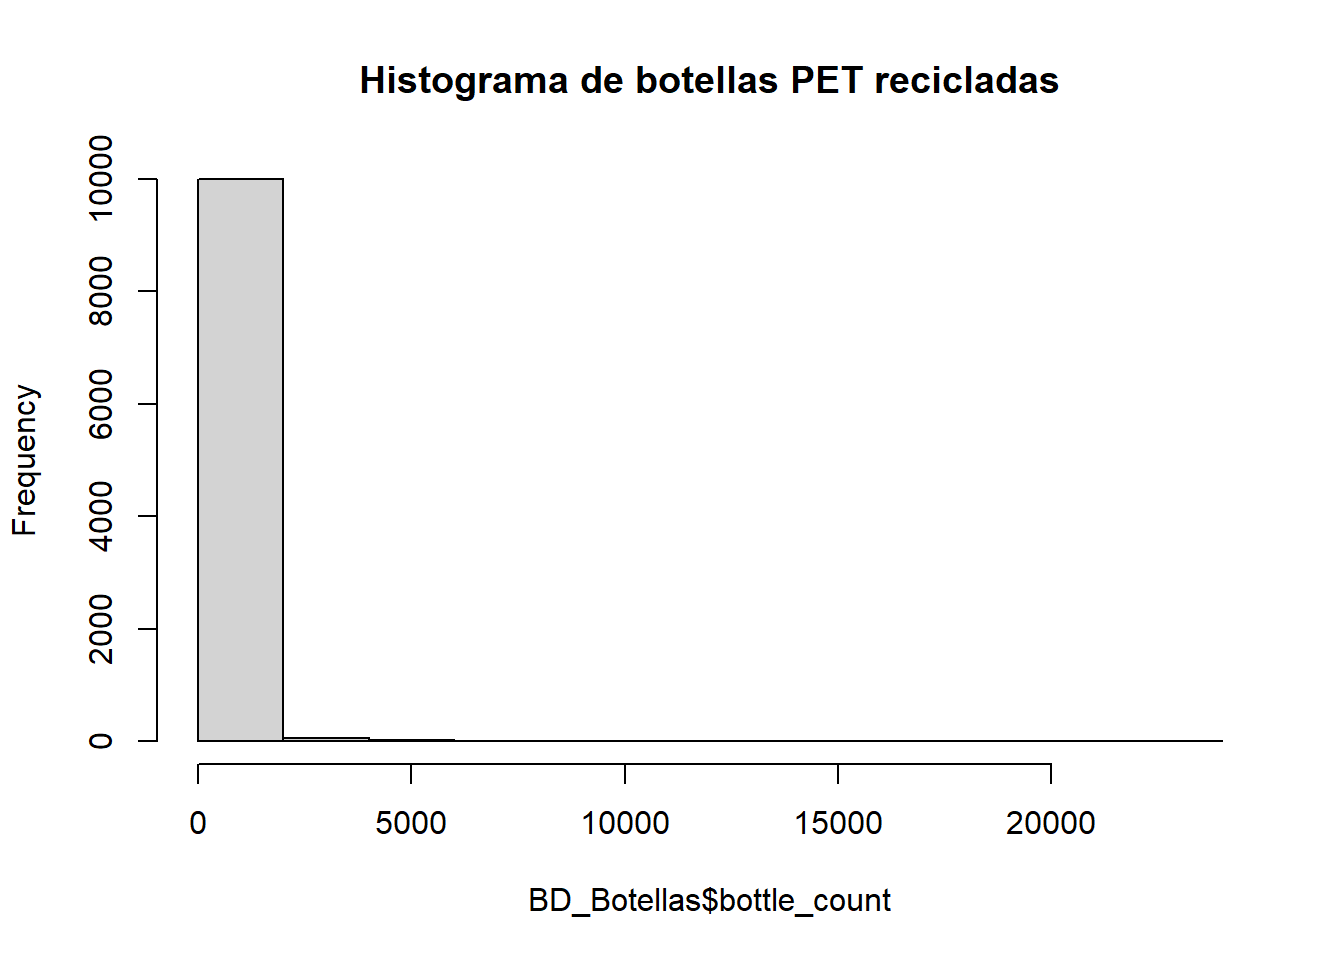
\includegraphics{analisis-baterias_files/figure-latex/unnamed-chunk-4-1.pdf}
Distribución de edades de la muestra

\begin{Shaded}
\begin{Highlighting}[]
\FunctionTok{hist}\NormalTok{(Muestra\_1005[ ,}\DecValTok{2}\NormalTok{],}
     \AttributeTok{breaks =} \DecValTok{3}\NormalTok{, }
     \AttributeTok{col=}\StringTok{"peachpuff"}\NormalTok{,}
     \AttributeTok{border=}\StringTok{"black"}\NormalTok{,}
     \AttributeTok{prob =} \ConstantTok{TRUE}\NormalTok{, }
     \AttributeTok{xlab =} \StringTok{"Edad"}\NormalTok{, }
     \AttributeTok{main =} \StringTok{"Distribución de edades"}\NormalTok{)}
\FunctionTok{lines}\NormalTok{(}\FunctionTok{density}\NormalTok{(Muestra\_1005[ ,}\DecValTok{2}\NormalTok{]),}
    \AttributeTok{lwd =} \DecValTok{2}\NormalTok{,}
    \AttributeTok{col=}\StringTok{"chocolate3"}
\NormalTok{                                            )}
\end{Highlighting}
\end{Shaded}

\includegraphics{analisis-baterias_files/figure-latex/unnamed-chunk-5-1.pdf}

\end{document}
